\chapter{\MakeUppercase{Кинематика конечностей робота}}
\section{Общее положение}
Изначально планировалось, что конечность робота в общем виде будет представлять манипулятор с тремя степенями свободы. Такая конструкция множество раз рассмотрена другими людьми, существует аналитическое решение прямой и обратной задачи.

Проблема такой кинематики в механической сложности ее реализации с точки зрения конструктора. Из-за особенностей и требований, описанный выше \fixme конструкция ноги получилась, как на рисунке ниже.
\begin{figure}[h]
    \centering
    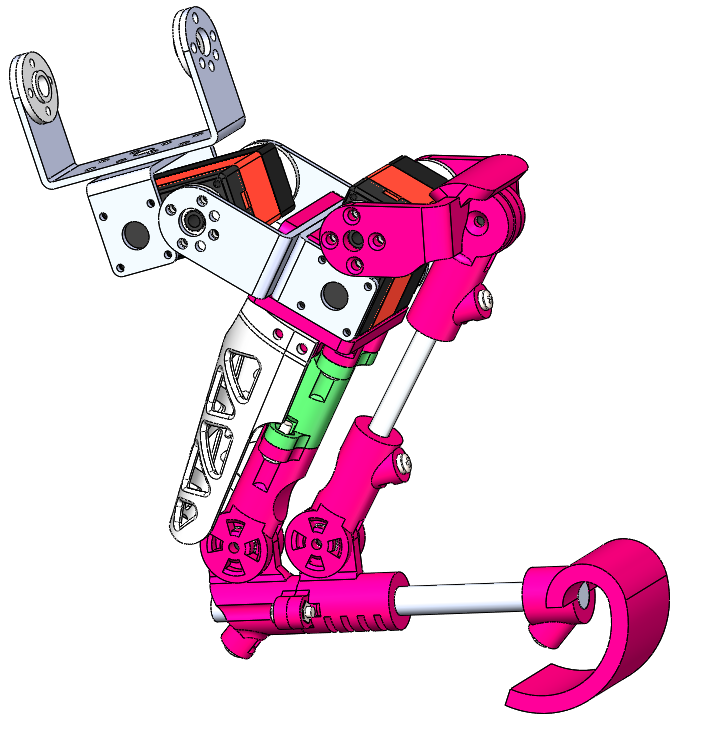
\includegraphics[scale=0.5]{chapter_kinematics/figure2.png}
    \caption{Чертеж конструкции ноги}
    \label{}
\end{figure}

Для упрощения понимания ниже приведена трехмерная кинематическая схема конечности.
\begin{figure}[h]
    \centering
    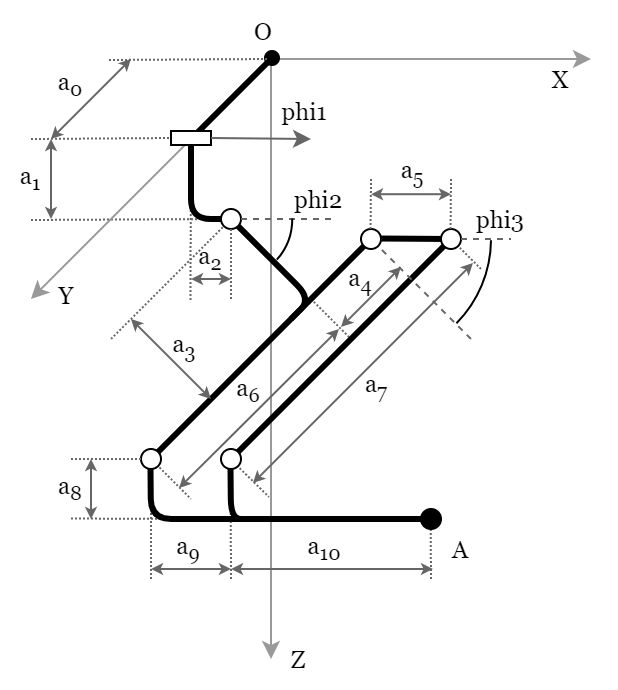
\includegraphics[scale=0.5]{chapter_kinematics/figure1.png}
    \caption{Трехмерная кинематическая схема ноги робота}
    \label{}
\end{figure}

В составе конечности присутствует непрямой кинематический четырехзвенник (три из четырех сторон имеют разные длины). Это усложнило кинематическую задачу, сделало ее менее тривиальной. Как оказалось далее, наличие четырехзвенной передачи сделало невозможным нахождение аналитического решения обратной задачи кинематики. 

На кинематической схеме отмечены величины, численные значения которых приведены ниже:
\begin{align*}
    a_0&=0.01 м \\
    a_1&=46.22 \times 10^{-3} м \\
    a_2&=20 \times 10^{-3} м \\
    a_3&=44 \times 10^{-3} м \\
    a_4&=20 \times 10^{-3} м \\
    a_5&=27 \times 10^{-3} м \\
    a_6&=87 \times 10^{-3} м \\
    a_7&=107 \times 10^{-3} м \\
    a_8&=12.62 \times 10^{-3} м \\
    a_9&=24.5 \times 10^{-3} м \\
    a_10&=110 \times 10^{-3} м
\end{align*}

Заметим, что расстояния $ a_5 $ и $ a_9 $ различаются! Диапазоны рабочих углов следующие:
\begin{align*}
    \varphi_1&=0 \dots \frac \pi 8 \\
    \varphi_2&=-\frac \pi 2 \dots 0 \\
    \varphi_3&=-\frac \pi 4 \dots \frac \pi 4
\end{align*}

Если зафиксировать первую степень свободы, $ \varphi_1 = 0 $, тогда рабочая область ноги будет лежать в плоскости $ XZ $. Выглядеть рабочая область с зафиксированным $ \varphi_1 $ будет следующим образом:
\begin{figure}[h]
    \centering
    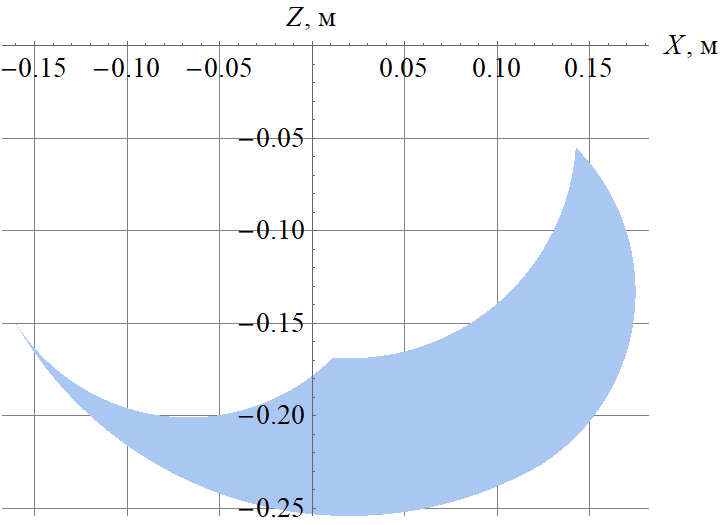
\includegraphics[scale=0.5]{chapter_kinematics/figure3.png}
    \caption{Сечение рабочей области конечности робота}
    \label{}
\end{figure}

Для построения рабочей области использованы уравнения прямой кинематики, которые будут выведены в пункте \ref{sec:direct_kinematics}.

\section{Общее решение четырёхзвенника}

При построении аналитического решения четырехзвенной передачи было важно подобрать функции так, чтобы для рабочих диапазонов углов $ \varphi_1, \varphi_2, \varphi_3 $ не возникало переходов через ноль, или через бесконечно большие числа. Важно избежать использования кусочных функций и условных операторов для упрощения программирования.
Малые диапазоны углов в рассматриваемой конечности упрощают эту задачу.

На рисунке \ref{fig:scheme_four} приведена схема четырехзвенника. Найдем зависимость $ \varphi_4 $ от $ \varphi_3 $. \fixme (надо на схеме выше показать phi4)
\begin{figure}[h]
    \centering
    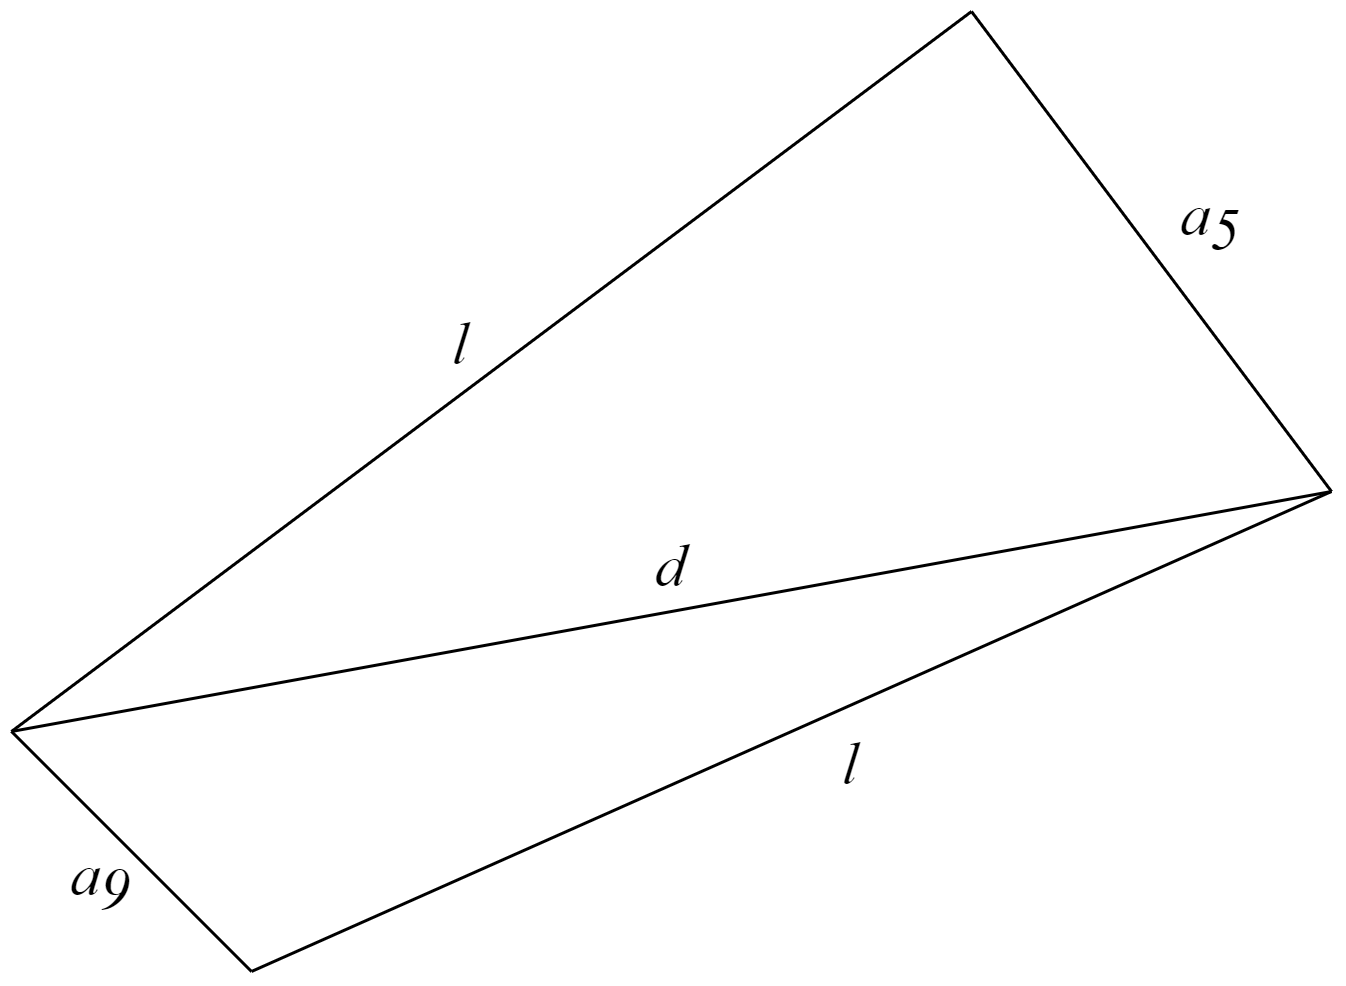
\includegraphics[scale=1]{chapter_kinematics/figure4.png}
    \caption{Четырехзвенник}
    \label{fig:scheme_four}
\end{figure}

Сначала найдем диагональ $d$ по теореме косинусов, для того чтобы выразить противолежащие углы:
\begin{align}
    d = \sqrt{a_5^2 + l^2 - 2a_5 l \cos(\varphi_3)} \label{eq:kin_1}
\end{align}

С помощью уравнения \ref{eq:kin_1} выразим углы:
\begin{align}
    \alpha &= \text{arccos}\left(\frac{d^2-a_9^2-l^2}{2 a_9 l}\right) \\
    \gamma &= \text{arcsin}\left(\frac{a_5}{d}\cos \varphi_3\right) \\
    \delta &= \text{arccos}\left(\frac{d^2+a_9^2-l^2}{2 a_9 l}\right)
\end{align}



\section{Прямая кинематика}\label{sec:direct_kinematics}
Используя найденную в пункте \fixme связь построим решение премой задачи кинематики.

\section{Обратная кинематика}


\section{Оптимизация численного решения обратной задачи}